\documentclass[letterpaper,11pt]{exam}
\usepackage{amssymb,amsmath,amsthm,mathtools}
\usepackage{pythonhighlight}

% https://www.overleaf.com/learn/latex/Hyperlinks
% https://www.lianxh.cn/details/904.html
\usepackage{hyperref}
\hypersetup{
    colorlinks=true,
    linkcolor=blue,
    filecolor=magenta,      
    urlcolor=cyan,
    pdftitle={Overleaf Example},
    pdfpagemode=FullScreen,
}
%

\usepackage{enumitem,amssymb}
\newlist{todolist}{itemize}{2}
\setlist[todolist]{label=$\square$}
\usepackage{pifont}
\newcommand{\cmark}{\ding{51}}%
\newcommand{\xmark}{\ding{55}}%
\newcommand{\done}{\rlap{$\square$}{\raisebox{2pt}{\large\hspace{1pt}\cmark}}%
\hspace{-2.5pt}}
\newcommand{\wontfix}{\rlap{$\square$}{\large\hspace{1pt}\xmark}}

\usepackage{indentfirst}


% \usepackage[UTF8]{ctex}
\usepackage[slantfont, boldfont]{xeCJK}

\usepackage{listings}
\usepackage{color}

\usepackage{xcolor}

% Define custom colors
\definecolor{mynote}{RGB}{255,0,255} % Color for notes
\definecolor{mynote2}{RGB}{0,155,155} % Color for notes


% Setup environment for notes
\newenvironment{mynotes}
{\begin{quote}\color{mynote}\textbf{Note:}}
{\end{quote}}

\newenvironment{mynotes2}
{\begin{quote}\color{mynote2}\textbf{Note:}}
{\end{quote}}




\definecolor{dkgreen}{rgb}{0,0.6,0}
\definecolor{gray}{rgb}{0.5,0.5,0.5}
\definecolor{mauve}{rgb}{0.58,0,0.82}

\lstset{frame=tb,
  language=Python,
  aboveskip=3mm,
  belowskip=3mm,
  showstringspaces=false,
  columns=flexible,
  basicstyle={\small\ttfamily},
  numbers=none,
  breaklines=true,
  numberstyle=\tiny\color{gray},
  keywordstyle=\color{blue},
  commentstyle=\color{dkgreen},
  stringstyle=\color{mauve},
  breakatwhitespace=true,
}



\newcommand{\num}{}
\newcommand{\topic}{ }
\newcommand{\coursenum}{15-645\quad}
\newcommand{\coursename}{\coursenum Database System}
\newcommand{\fullname}{Siqi Guo}
\newcommand{\andrew}{siqiguo}
\setlength{\parindent}{0pt} %don't indent first line of paragraph

\pagestyle{headandfoot}
\runningheadrule
\firstpageheader{}{}{}
\runningheader{\fullname}{\coursenum\ \textbf{\topic}}{\andrew}
\firstpagefooter{}{\thepage}{}
\runningfooter{}{\thepage}{}
\extrawidth{.5in}\extraheadheight{-.25in}

\newcommand{\soln}[1]{\begin{solution}#1\end{solution}}

\begin{document}
\begin{center}
    {\LARGE\coursename\par}
    \fullname \quad (\andrew) \hfill \today
\end{center}

\section*{Course Overview}


In the context of the Distributed System 15-640, we want to give the illusion that we operate the file system in local machine, even if it's actually operated on the remote server.

While, here, DBMS wants to give the illusion that we are operating with the database entirely in memory.

\vspace*{1em}
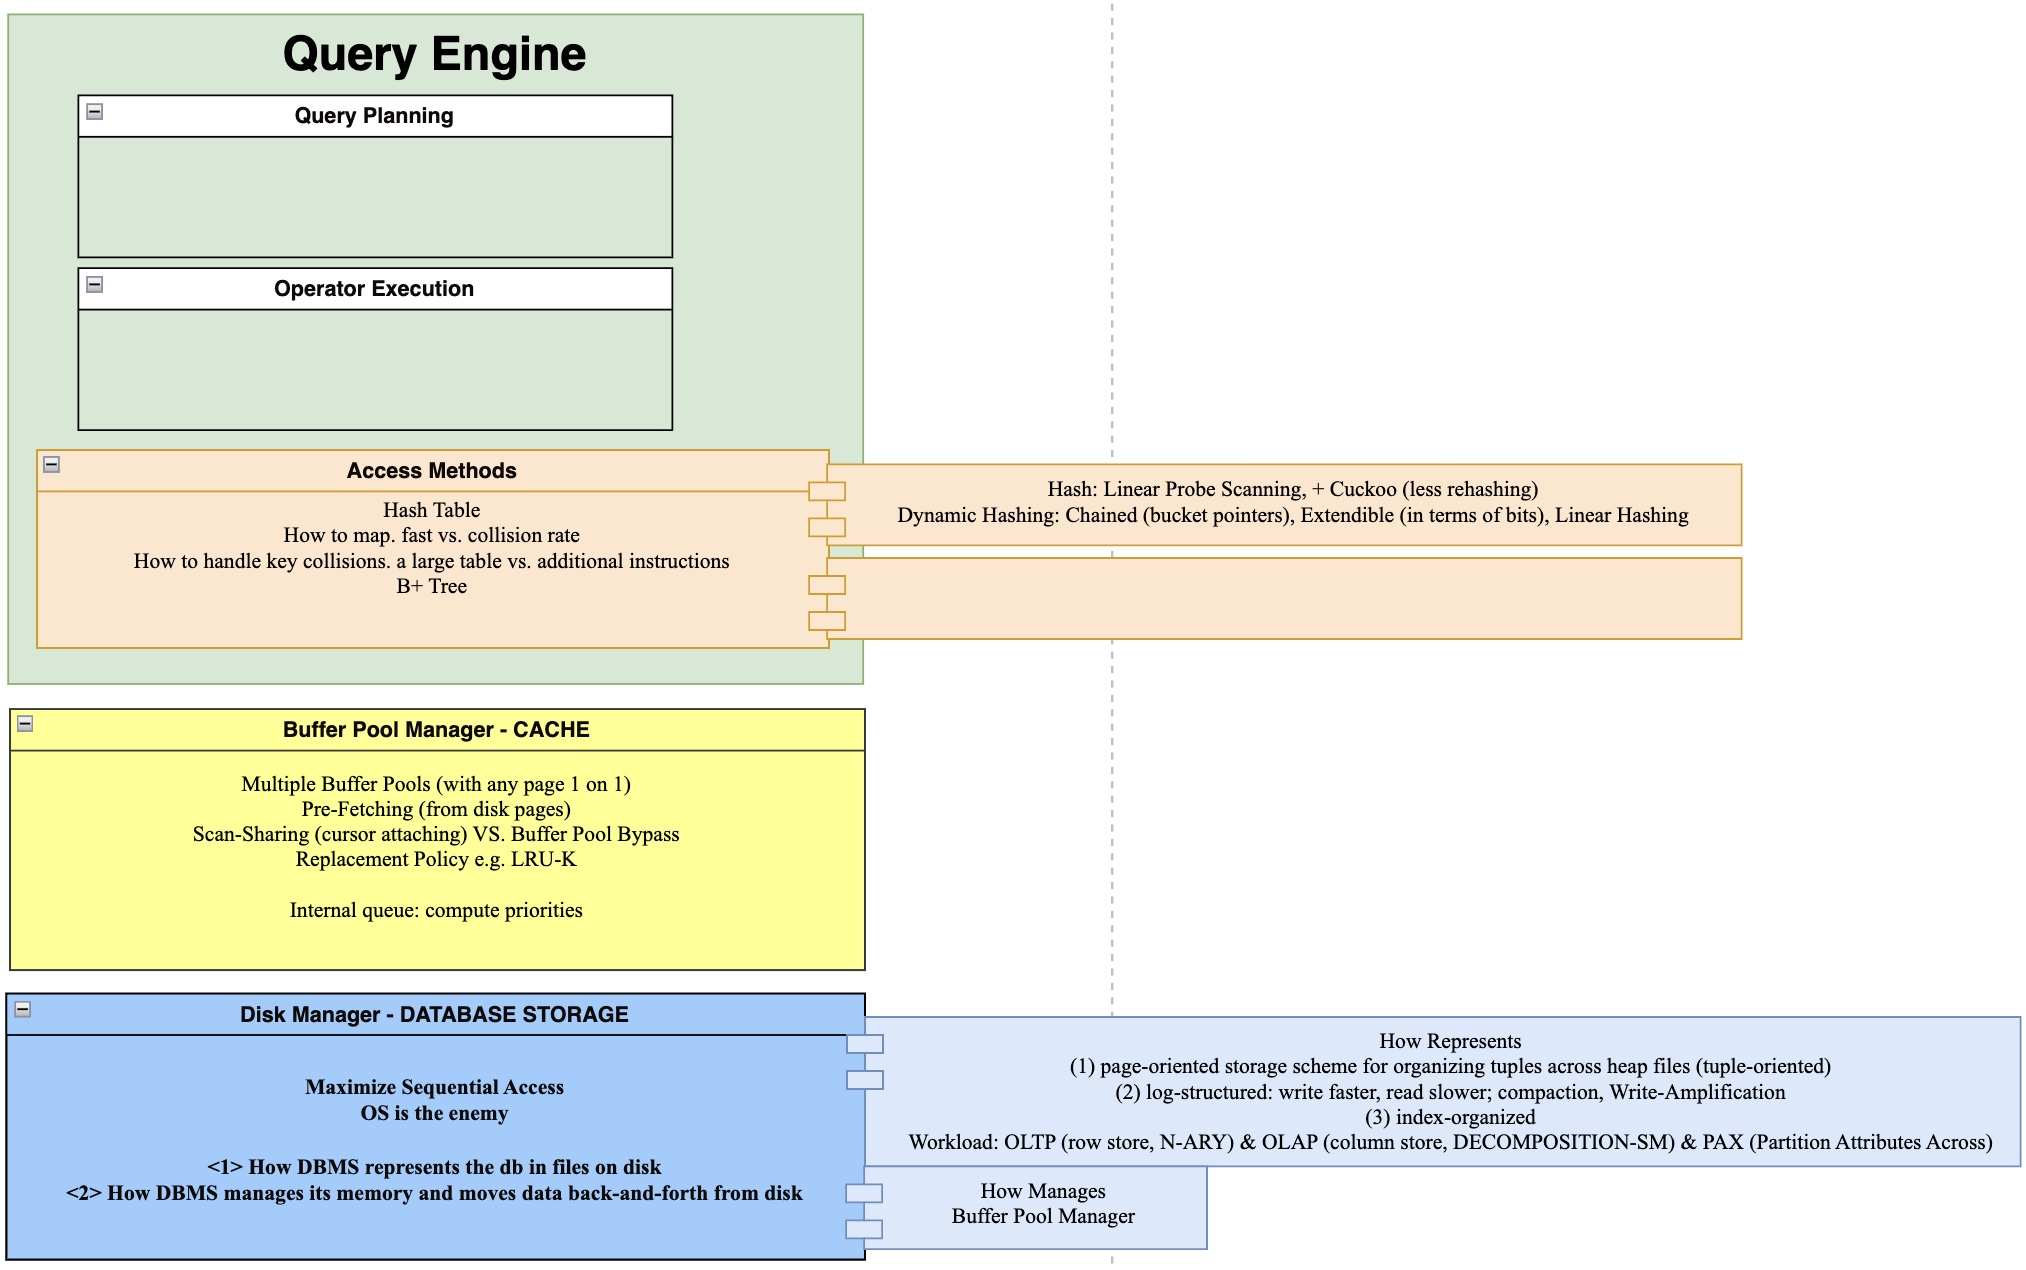
\includegraphics[width=\textwidth]{../diagram/diagram_1.jpg}

% \subsection*{title}
% The communication between the proxy and the server is based on JAVA RMI Interface. The server implemented those functions which would work as stubs in the proxy. Each time, the proxy would make RPC calls to the server, just like what the clients did in the project one. \\

% The protocol between the proxy and the server includes check-on-use and last-close-win strategies. Generally, when the proxy opens a file, it would request that file's metadata and check them. 
% The reason I used a metadata RPC request is to decrease the RPC call times. Without this sturcturized metadata, the proxy have to make more RPC calls to get the information of whether the file exists, whether the path is actually a directory, what is the file's length, and what is the file's UUID. \\   

% Then, with the metadata checking, if the operation is invalid, this session would return ERROR. Then, the proxy would check if the file is stale. 
% If the file is stale in its cache, the proxy would request the file from the server and update its cache, otherwise, the proxy would only use the cached file to continue system calls. Here, the UUID is used to control the version of those files, and file length and isFirstChunk flag are used to transfer the chunked data between the proxy and the server. 

% \subsection{Consistency Model}
% Regarding the Consistency Model, I implement the open-close session semantics. \\

% For each open operation, the proxy would check the file's version on the server. The server only have one version for each file and only update the file and its version when there is a close operation in the proxy and this proxy is trying to update the file to the server. \\

% However, the proxy needs to manage all versions of the file in its cache. Because a writer's writing should be invisible to other reader clients in this proxy, I give each writer client a unique write copy. Once they completed their writing, the proxy would update the dirty flag, making this file enable to be updated to the server when the writer closes. After updating, this write copy would be deleted from the cache. \\

% Besides, the stale file with no one using would be deleted as well at each open beginning to deduplicate the cache files. Whether a file is used or not is determined by the file's reference count number. \\

% \subsection{LRU Replacement \& Cache Freshness}
% When it comes to LRU replacement, first, I implement a doubly linked list to manage the file's data in the cache. Each node in this linked list consists of the file object itself, some necessary parts of a file's metadata, predecessor, and successor pointers (which are also the LRU nodes). When a file is used, and it should be updated at the end of close operation by LRU policy, this corresponding node would be moved to the head of the list. When the cache is full, and it needs to evict, the cache will evict the nodes from the tail's previous node (at the end of the list) when they are not used, until the cache has free space. \\
% I use a concurrent hash map to store the mapping between the path with version and the LRU linked list node. In this case, the cache could deal with different versions of a file. \\

% \subsection{Concurrency}
% The concurrency for proxy to dealing with the clients is implemented by FileHandler provided by the project. The proxy uses ConcurrentHashMap to store the mapping between the file descriptor and the File, cache uses ConcurrentHashMap to store LRU linked list node, and the server also uses ConcurrentHashMap to store the mapping between file version and file path and the mapping between the file path and read-write lock. In this way, most concurrency in this project are implemented by the property of ConcurrentHashMap. I made a trade-off to get the efficiency but lose some flexible to use the lock by myself. However, only using ConcurrentHashMap could not solve all concurrency issue. \\

% I also use \texttt{synchronized} for cache insertion, eviction, and deletion (otherwise LRU Test 2 would fail because it tested the case that a client sends a lot of same-file read request, which will fill the cache if there is no synchronized processing in cache). I also use \texttt{ReentrantReadWriteLock} for the file-level lock in the server, which I will explain in the next section. \\ 

% \subsection{Some Interesting Highlights}
% Regarding the chunking section, I used a flag \texttt{isFirstChunk} (inspired by one of the TAs in the OH) to control the file read-write lock in the server. 
% In this way, server could provide file-level lock and unlock in case of read-write toggling and conflicts when there are many chunks and there is a long time to transfer the data between the proxy and the server. When the first chunk flag is true, and the proxy would make the server lock the read of write operations until the end of those chunks. \\

% Secondly, I found that write copy have to be done in the open operation, otherwise, it would cause bugs during many write chunk operations if I choose copy the file in the write operation. However, it makes sense to me later that if a writer opens a file with write permission, I have to provide the write-copy no matter whether the writer would write or not. 
% This implementation requires me to check the cache size after each write operation because I only copy the file once and the cache size has to be checked to avoid the cache overflow. (given write would change the size of the file in the cache.) \\

% Last, I use a flag to distinguish whether a delete operation is for a stale file or for the unlink system call. The reason is if a file is stale and needs to be deleted, I could delay this delete operation if this file is being used and skip this delete in the cache ("delete" checked in the open operation, delete happened once this stale file is not being used any more). However, if it is an unlink, I need to block other operations with a while loop until this file is not being used any more and delete it in the cache. \\

\end{document}